\section{学位论文排版}
\subsection{\ThuThesis 清华大学学位论文模板}

\begin{frame}{\ThuThesis}
  \framesubtitle{清华大学学位论文 \LaTeX{} 模板}
  \begin{itemize}
  \item 最早:王磊~(2004.4)
  \item 2005 年:薛瑞尼
  \item 最新正式版:5.3.1 (2016-03-20)
  \item 最近更新:2016/03/25
  \item 全面支持本科、硕士、博士、博士后论文格式
  \end{itemize}
  \begin{figure}[htbp]
    \centering
    
\includegraphics[height=.4\textheight]{cover-bachelor-crop.pdf}\hfill
    
\includegraphics[height=.4\textheight]{cover-master-crop.pdf}\hfill
    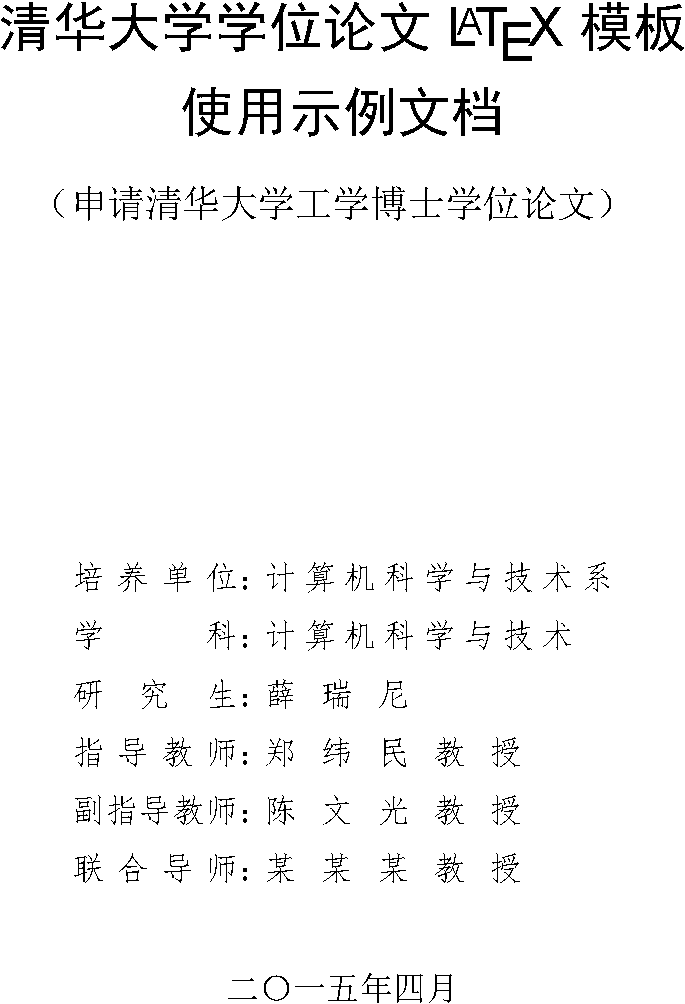
\includegraphics[height=.4\textheight]{cover-doctor-crop.pdf}\hfill
    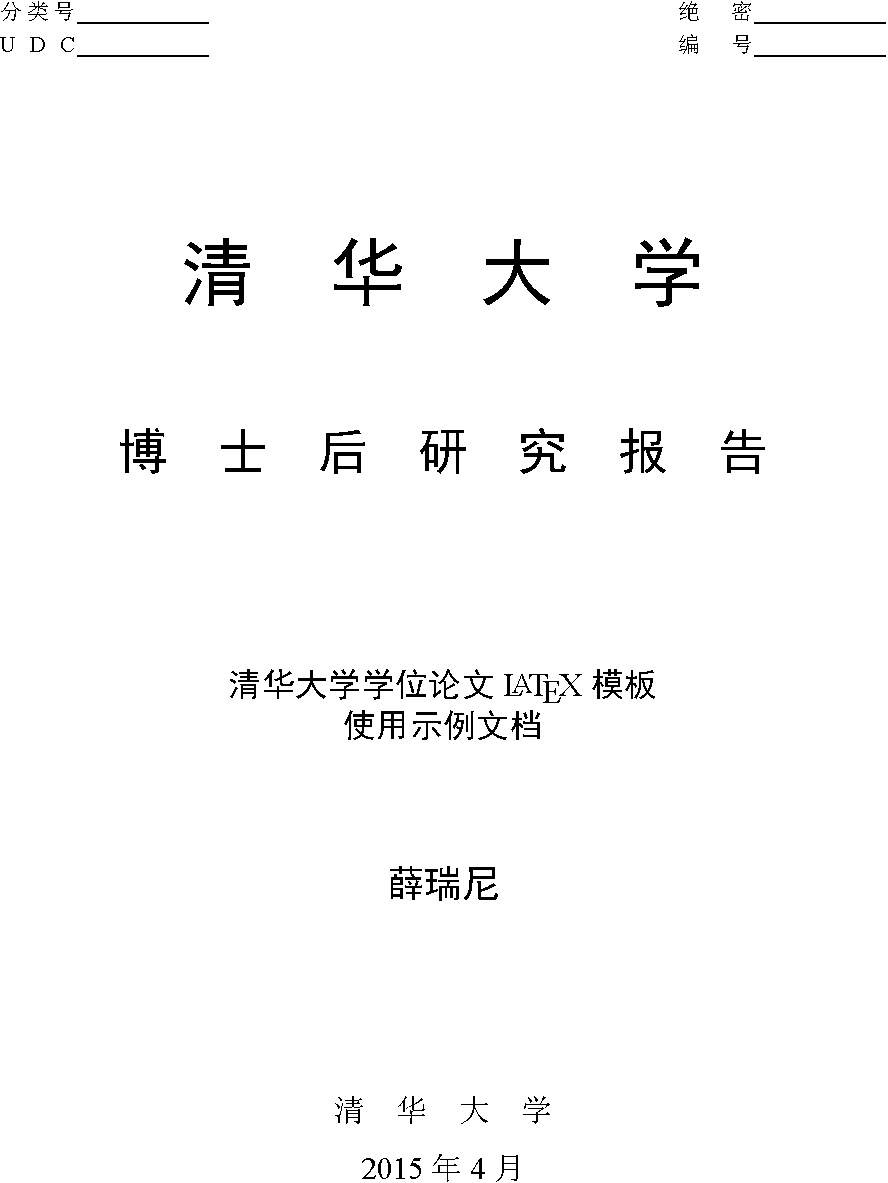
\includegraphics[height=.4\textheight]{cover-postdoctor-crop.pdf}
  \end{figure}
\end{frame}

\begin{frame}{安装\ThuThesis}

\begin{itemize}
	\item \TL 和 C\TeX 清华特别版已经带了,一般不用特地装
    \item 也可以到 CTAN 自行下载
	\item 但是每年都会更新,有时需要装最新开发版……
\end{itemize}
	

\end{frame}

\begin{frame}{安装\ThuThesis}
      \begin{columns}
        \begin{column}{.7\textwidth}
  \begin{itemize}
    \item 下载最新开发版
      \begin{itemize}
        \item \url{https://github.com/xueruini/thuthesis}
        \item 右边栏
          \href{https://github.com/xueruini/thuthesis/archive/master.zip}%
          {Download ZIP} 按钮
        %\item Git 用户还可以直接克隆仓库
      \end{itemize}
    \item 下载最新正式版
      \begin{itemize}
        \item \url{http://mirrors.ctan.org/macros/latex/contrib/thuthesis.zip}
      \end{itemize}
  \end{itemize}
        \end{column}
        \begin{column}{.3\textwidth}
          \begin{figure}[htbp]
            \centering
            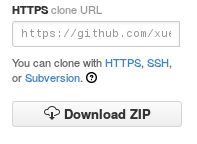
\includegraphics[width=.8\textwidth]{thuthesis-download.png}
          \end{figure}
        \end{column}
      \end{columns}
  \begin{itemize}
    \item 安装
      \begin{itemize}
        \item 解压缩看文档 \texttt{README.md}
        \item 模板文档类:XeLaTeX 编译一次 \texttt{thuthesis.ins} $\Rightarrow$
          \texttt{thuthesis.cls} 和 \texttt{thuthesis.cfg}
		\item 用户手册:XeLaTeX 编译两次 \texttt{thuthesis.dtx} $\Rightarrow$
          \texttt{thuthesis.pdf}
        \item 论文示例:对 \texttt{main.tex} 执行一次 XeLaTeX,一次 BibTeX,再两次
          XeLaTeX
        \item 可使用或参考附带的 Makefile
      \end{itemize}
  \end{itemize}
\end{frame}

\begin{frame}[fragile]{论文选项}
\begin{description}
\item[bachelor] 我要写本科论文
  \begin{lstlisting}[basicstyle=\ttfamily]
\documentclass[bachelor]{thuthesis}
  \end{lstlisting}
\item[master] 我要写硕士论文
  \begin{lstlisting}[basicstyle=\ttfamily]
\documentclass[master]{thuthesis}
  \end{lstlisting}
\item[doctor] 我要写博士论文
  \begin{lstlisting}[basicstyle=\ttfamily]
\documentclass[doctor]{thuthesis}
  \end{lstlisting}
\item[secret] 论文有保密要求
  \begin{lstlisting}[basicstyle=\ttfamily]
\documentclass[doctor, secret]{thuthesis}
\secretlevel{机密}
\secretyear{2010}
  \end{lstlisting}
\end{description}
\end{frame}

\begin{frame}{封面}
  \begin{table}[h]
    \centering
\footnotesize
  \begin{tabular}{lll}
    命令作用 & 中文命令 & 英文命令 \\\hline\hline
  论文标题 & \cmd{ctitle} &\cmd{etitle}\\
  作者姓名&  \cmd{cauthor} &\cmd{eauthor}\\
  申请学位名称 & \cmd{cdegree}&\cmd{edegree}\\
  院系名称 & \cmd{cdepartment} & \cmd{edepartment}\\
  专业名称 & \cmd{cmajor} & \cmd{emajor}\\
  导师 & \cmd{csupervisor} & \cmd{esupervisor}\\
  副导师 & \cmd{cassosupervisor} & \cmd{eassosupervisor}\\
  联合导师 & \cmd{ccosupervisor} & \cmd{ecosupervisor}\\
  日期 & \cmd{cdate} & \cmd{edate}\\
  摘要 & \cmd{cabstract} & \cmd{eabstract}\\
  关键词 & \cmd{ckeywords} & \cmd{ekeywords}\\\hline
  \end{tabular}
  \end{table}
\end{frame}

\begin{frame}{数学}
  \begin{itemize}
    \item 公式示例:\nolinkurl{data/chap01.tex}
    \item \ThuThesis{} 定义了常用的数学环境
      \begin{table}[h]
        \centering
    \begin{tabular}{lllll}\hline
axiom & theorem & definition & proposition & lemma \\
公理 & 定理 & 定义 & 命题 & 引理 \\\hline
proof & corollary & example & exercise &\\
证明 & 推论 & 例子& 练习 &\\\hline
    \end{tabular}
      \end{table}
  \end{itemize}
\end{frame}

\begin{frame}[fragile]{参考文献}
  \begin{itemize}
    \item 推荐 \BibTeX
      \begin{itemize}
        \item 使用文献管理软件导出 bib 文件
          \begin{itemize}
            \item Menderley, NoteExpress
          \end{itemize}
        \item 使用 bibtex 生成参考文献列表
        \item bst 参考文献样式文件:\texttt{thubib.bst}
      \end{itemize}
    \item 学校要求两种引用方式:
      \begin{itemize}
        \item 上标模式:如``在许多文献\textsuperscript{[12,13]}中……''
        \begin{lstlisting}[basicstyle=\ttfamily]
  \cite{key12, key13}
        \end{lstlisting}
      \item 正文模式:如``文献~[14] 证明了……''
        \begin{lstlisting}[basicstyle=\ttfamily]
  \inlinecite{key14}
        \end{lstlisting}
      \end{itemize}
    \end{itemize}
\end{frame}

\begin{frame}{作图}
  \begin{columns}[c]
    \begin{column}{.5\textwidth}
  \begin{itemize}
  \item 矢量图 eps, ps, pdf
    \begin{itemize}
    \item \MP, pstricks, pgf $\ldots$
    \item Xfig, Dia, \alert{Visio}, \alert{Inkscape} $\ldots$
    \item Matlab / Excel 等保存为 pdf
    \end{itemize}
  \item 标量图 png, jpg, tiff $\ldots$
    \begin{itemize}
      \item 提高清晰度,避免发虚
    \end{itemize}
  \item 转化
    \begin{itemize}
    \item 虚拟打印机
    \item ImageMagick
    \item epstopdf
    \item pdfcrop
    \end{itemize}
  \end{itemize}
    \end{column}
    \begin{column}{.4\textwidth}
\begin{figure}[h]
  \centering
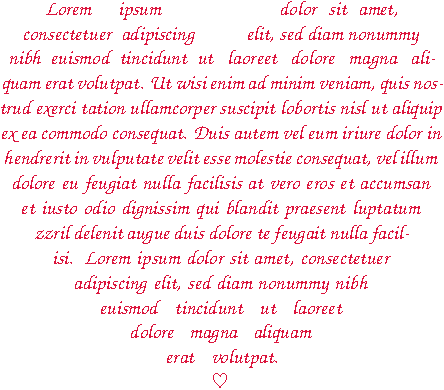
\includegraphics[height=.3\textheight]{shapepar.pdf}\\\vspace{1cm}
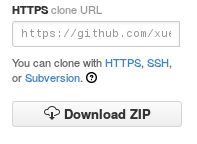
\includegraphics[height=.3\textheight]{thuthesis-download.png}
\end{figure}
    \end{column}
  \end{columns}
\end{frame}

%%% vim: set sw=2 isk+=\: et tw=80 cc=+1 formatoptions+=mM:
